
\makequotation{It is practically impossible to teach good programming to
  students that have had a prior exposure to BASIC: as potential
  programmers they are mentally mutilated beyond hope of
  regeneration.}{Edsger W. Dijkstra, Turing Award winner~\cite{dijkstra-truths}}

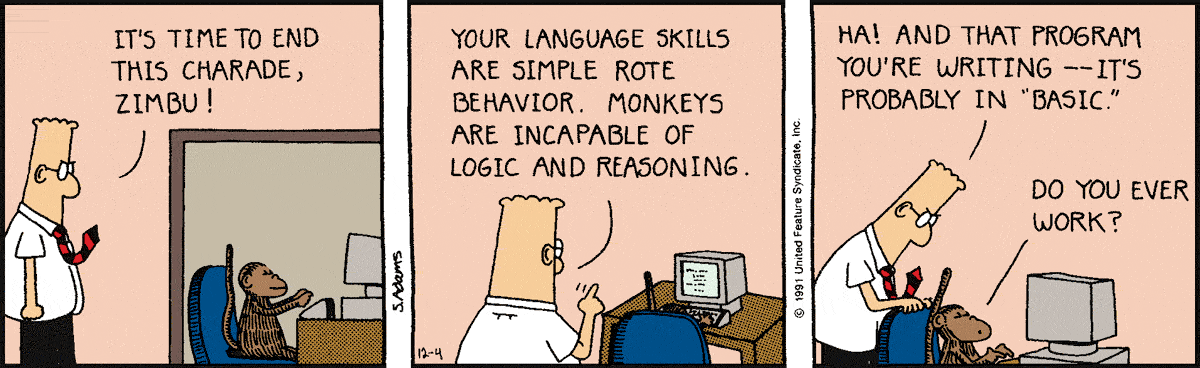
\includegraphics[width=\textwidth]{figs/dilbert-1991-12-04.png}

The early democratization of computing owes its success to three
factors.  The first, of course, is the 1971 invention of the 4004 microprocessor
by Ted Hoff and others at 
Intel; the 4004 is arguably the distant ancestor of the x86
architecture.
The second factor is the ability of the microprocessor industry
to exploit Moore's Law,
increasing the performance of microprocessors by a factor of over 1,000
since 1971, and  increasing
price/performance by many orders of magnitude.
The third factor is the invention and rapid dissemination of the
high-level introductory programming language BASIC.

Before universities had computers that were widely accessible to students, BASIC
provided a kinder, gentler introduction to computing suitable for
everyone, especially nontechnical majors.
Before there was such a thing as a PC software industry, 
BASIC allowed early hobbyists to quickly get started writing their own
programs.
Before computer games became a multibillion-dollar industry, beginning
programmers and hobbyists were writing their own games in BASIC, to
exploit the rapidly-developing capabilities of graphics and sound on
early PCs. 
Much of the other software that fueled the PC revolution---online
bulletin boards, simple utilities, small-business software---was written
in BASIC. 
As science fiction author David Brin has written~\cite{why_johnny_cant_code},
despite its flaws, BASIC
was sufficiently nonthreatening to introduce an entire generation of
newbies to the joy of programming.

Today's world-class universities boast that over 90\% of all
undergraduates are exposed to introductory programming, and movements
like ``CS for all'' and sites like \T{code.org} aim to expose everyone
to coding.
Dartmouth College, where BASIC was invented, had largely
achieved this by 1971 on its campus~\cite{man_and_computer} by implementing the
farsighted vision of BASIC's creators.
Together with a wide cast of characters including Bob
Albrecht, David Ahl, Paul Allen, Dennis Allison, Bill Gates, Chuck
Peddle, Ed Roberts, Li-Chen Wang, Steve Wozniak, and the companies and
institutions where they worked, BASIC introduced an entire generation
of hobbyist programmers to the joy of programming.

Yet quotes like Dijkstra's show that despite its pivotal role in the PC
revolution, BASIC is probably one of the most maligned programming
languages to achieve widespread use.  It's time the true story of
BASIC's influence was told.
